
\begin{frame}{‌جستجوی دودویی}
\begin{itemize}\itemr
\item[-]
برای جستجوی یک مقدار در یک آرایه باید همهٔ عناصر آرایه را یک‌به‌یک بررسی کنیم. این جستجو برای یک آرایه با
\m{n}
عنصر در زمان
\m{O(n)}
انجام می‌شود.
\item[-]
حال فرض می‌کنیم می‌خواهیم یک مقدار را در یک آرایه مرتب شده پیدا کنیم.
\item[-]
برای این کار می‌توانیم از یک الگوریتم تقسیم و حل به نام جستجوی دودویی
\fn{1}{binary search}
استفاده کنیم.
\end{itemize}
\end{frame}


\begin{frame}{‌جستجوی دودویی}
\begin{itemize}\itemr
\item[-]
الگوریتم تقسیم و حل آرایه را به دو قسمت تقسیم می‌کند. برای جستجوی مقدار
\code{x}
در آرایه
\code{A}
، ابتدا مقدار
\code{x}
با عنصر وسط آرایه یعنی
\code{A[n/2]}
مقایسه می‌شود. اگر
\code{x}
برابر با مقدار وسط آرایه بود، مقدار مورد نظر یافته شده است. اگر
\code{x}
کوچکتر از عنصر وسط آرایه بود، باید
\code{x}
را در نیمه اول آرایه یعنی\\
\code{A[1:n/2-1]}
جستجو کنیم. در غیراینصورت باید
\code{x}
را در نیمه دوم آرایه یعنی
\code{A[n/2+1:n]}
جستجو کنیم. این روند را برای زیر آرایه‌ها ادامه می‌دهیم تا یا
\code{x}
یافته شود یا مشخص شود که
\code{x}
در آرایه وجود ندارد.
\end{itemize}
\end{frame}


\begin{frame}{‌جستجوی دودویی}
\begin{itemize}\itemr
\item[-]
بنابراین مراحل انجام جستجوی دودویی به صورت زیر است.
\item[۱.]
تقسیم : برای پیدا کردن مقدار
\code{x}
در آرایه
\code{A[low:high]}
قرار می‌دهیم
\code{mid=$\lfloor$(low + high)/2$\rfloor$} .
اگر
\code{A[mid]}
برابر با
\code{x}
بود به نتیجه رسیده‌ایم در غیراینصورت آرایه را به دو قسمت
\code{A[low:mid-1]}
و
\code{A[mid+1:high]}
تقسیم می‌کنیم. این تقسیم تنها در صورتی می‌تواند انجام شود که
\code{high}
از
\code{low}
بزرگ‌تر باشد.
\item[۲.]
حل : در صورتی که مقدار
\code{x}
از
\code{A[mid]}
کوچکتر بود، الگوریتم جستجو برای
\code{A[low:mid-1]}
فراخوانی می‌شود، در غیراینصورت برای
\code{A[mid+1:high]}
فراخوانی می‌شود.
\item[۳.]
ترکیب : در گام ترکیب هیچ عملیاتی انجام نمی‌شود.
\end{itemize}
\end{frame}


\begin{frame}{‌جستجوی دودویی}
\begin{itemize}\itemr
\item[-]
برای پیدا کردن عدد ۱۸ در آرایهٔ زیر، الگوریتم به صورت زیر عمل می‌کند.
\begin{figure}
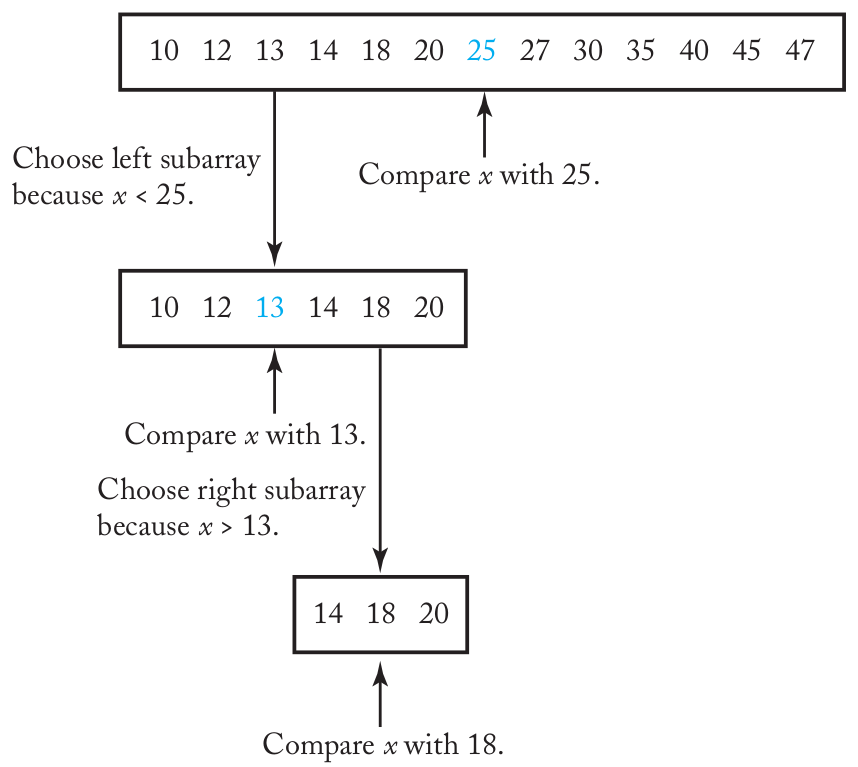
\includegraphics[width=0.55\textwidth]{figs/chap03/binarysearch2-1}
\end{figure}
\end{itemize}
\end{frame}


\begin{frame}{‌جستجوی دودویی}
\begin{itemize}\itemr
\item[-]
الگوریتم جستجوی دودویی به صورت زیر است.
\begin{algorithm}[H]\alglr
  \caption{‌Binary Search} 
  \begin{algorithmic}[1]
   \Func{BinarySearch}{A, x, low, high}
   \If{(low > high)}
        \State \Return -‌1
    \EndIf
    \State mid = $\lfloor$(low + high)/2$\rfloor$
    \If{(x == A[mid])}
         \State \Return mid
     \EndIf
     \If{(x < A[mid])}
          \State \Return BinarySearch (A, x, low, mid-1)
      \Else
          \State \Return BinarySearch (A, x, mid+1, high)
      \EndIf                          
  \end{algorithmic}
  \label{alg:merge}
\end{algorithm}
\item[-]
برای جستجوی مقدار
\code{x}
جستجوی دودویی باید به صورت
\code{BinarySearch(A, x, 1, n)}
فراخوانی شود.
\end{itemize}
\end{frame}



\begin{frame}{‌جستجوی دودویی}
\begin{itemize}\itemr
\item[-]
در تقسیم یک آرایه به دو قسمت صرفا یک عملیات تقسیم انجام می‌شود. بنابراین
\m{D(n) = O(1)}
. تقسیم آرایه در زمان ثابت انجام می‌شود.
\item[-]
بنابراین زمان اجرای الگوریتم جستجوی دودویی برای آرایه با
\m{n}
عنصر برابر است با زمان اجرای الگوریتم برای آرایه‌ای با
\m{n/2}
عنصر به علاوه یک زمان ثابت.
\item[-]
می‌توانیم بنویسیم
\m{T(n) = T(\frac{n}{2}) + O(1)}
و
\m{T(1) = 1}
\item[-]
با حل این رابطه بازگشتی به دست می‌آوریم
\m{T(n) = O(\lg n)}.
\end{itemize}
\end{frame}
